
\section*{\color{white}Introduzione}

\begin{frame}{Collaboratori}

  \begin{itemize}
  \item Dott. Carlo Battilana, titolare modulo laboratorio A-L
  \item Dott. Fabio Ferrari, titolare modulo laboratorio M-Z
  \item Dott. Giulio Colombini, tutor
  \item Dott. Simone Rossi Tisbeni, tutor
  \end{itemize}

\end{frame}

% sondaggio
\begin{frame}
  \begin{center}
    \vfill
    \url{https://forms.office.com/e/D89Yjd05Gz}
    \vfill
    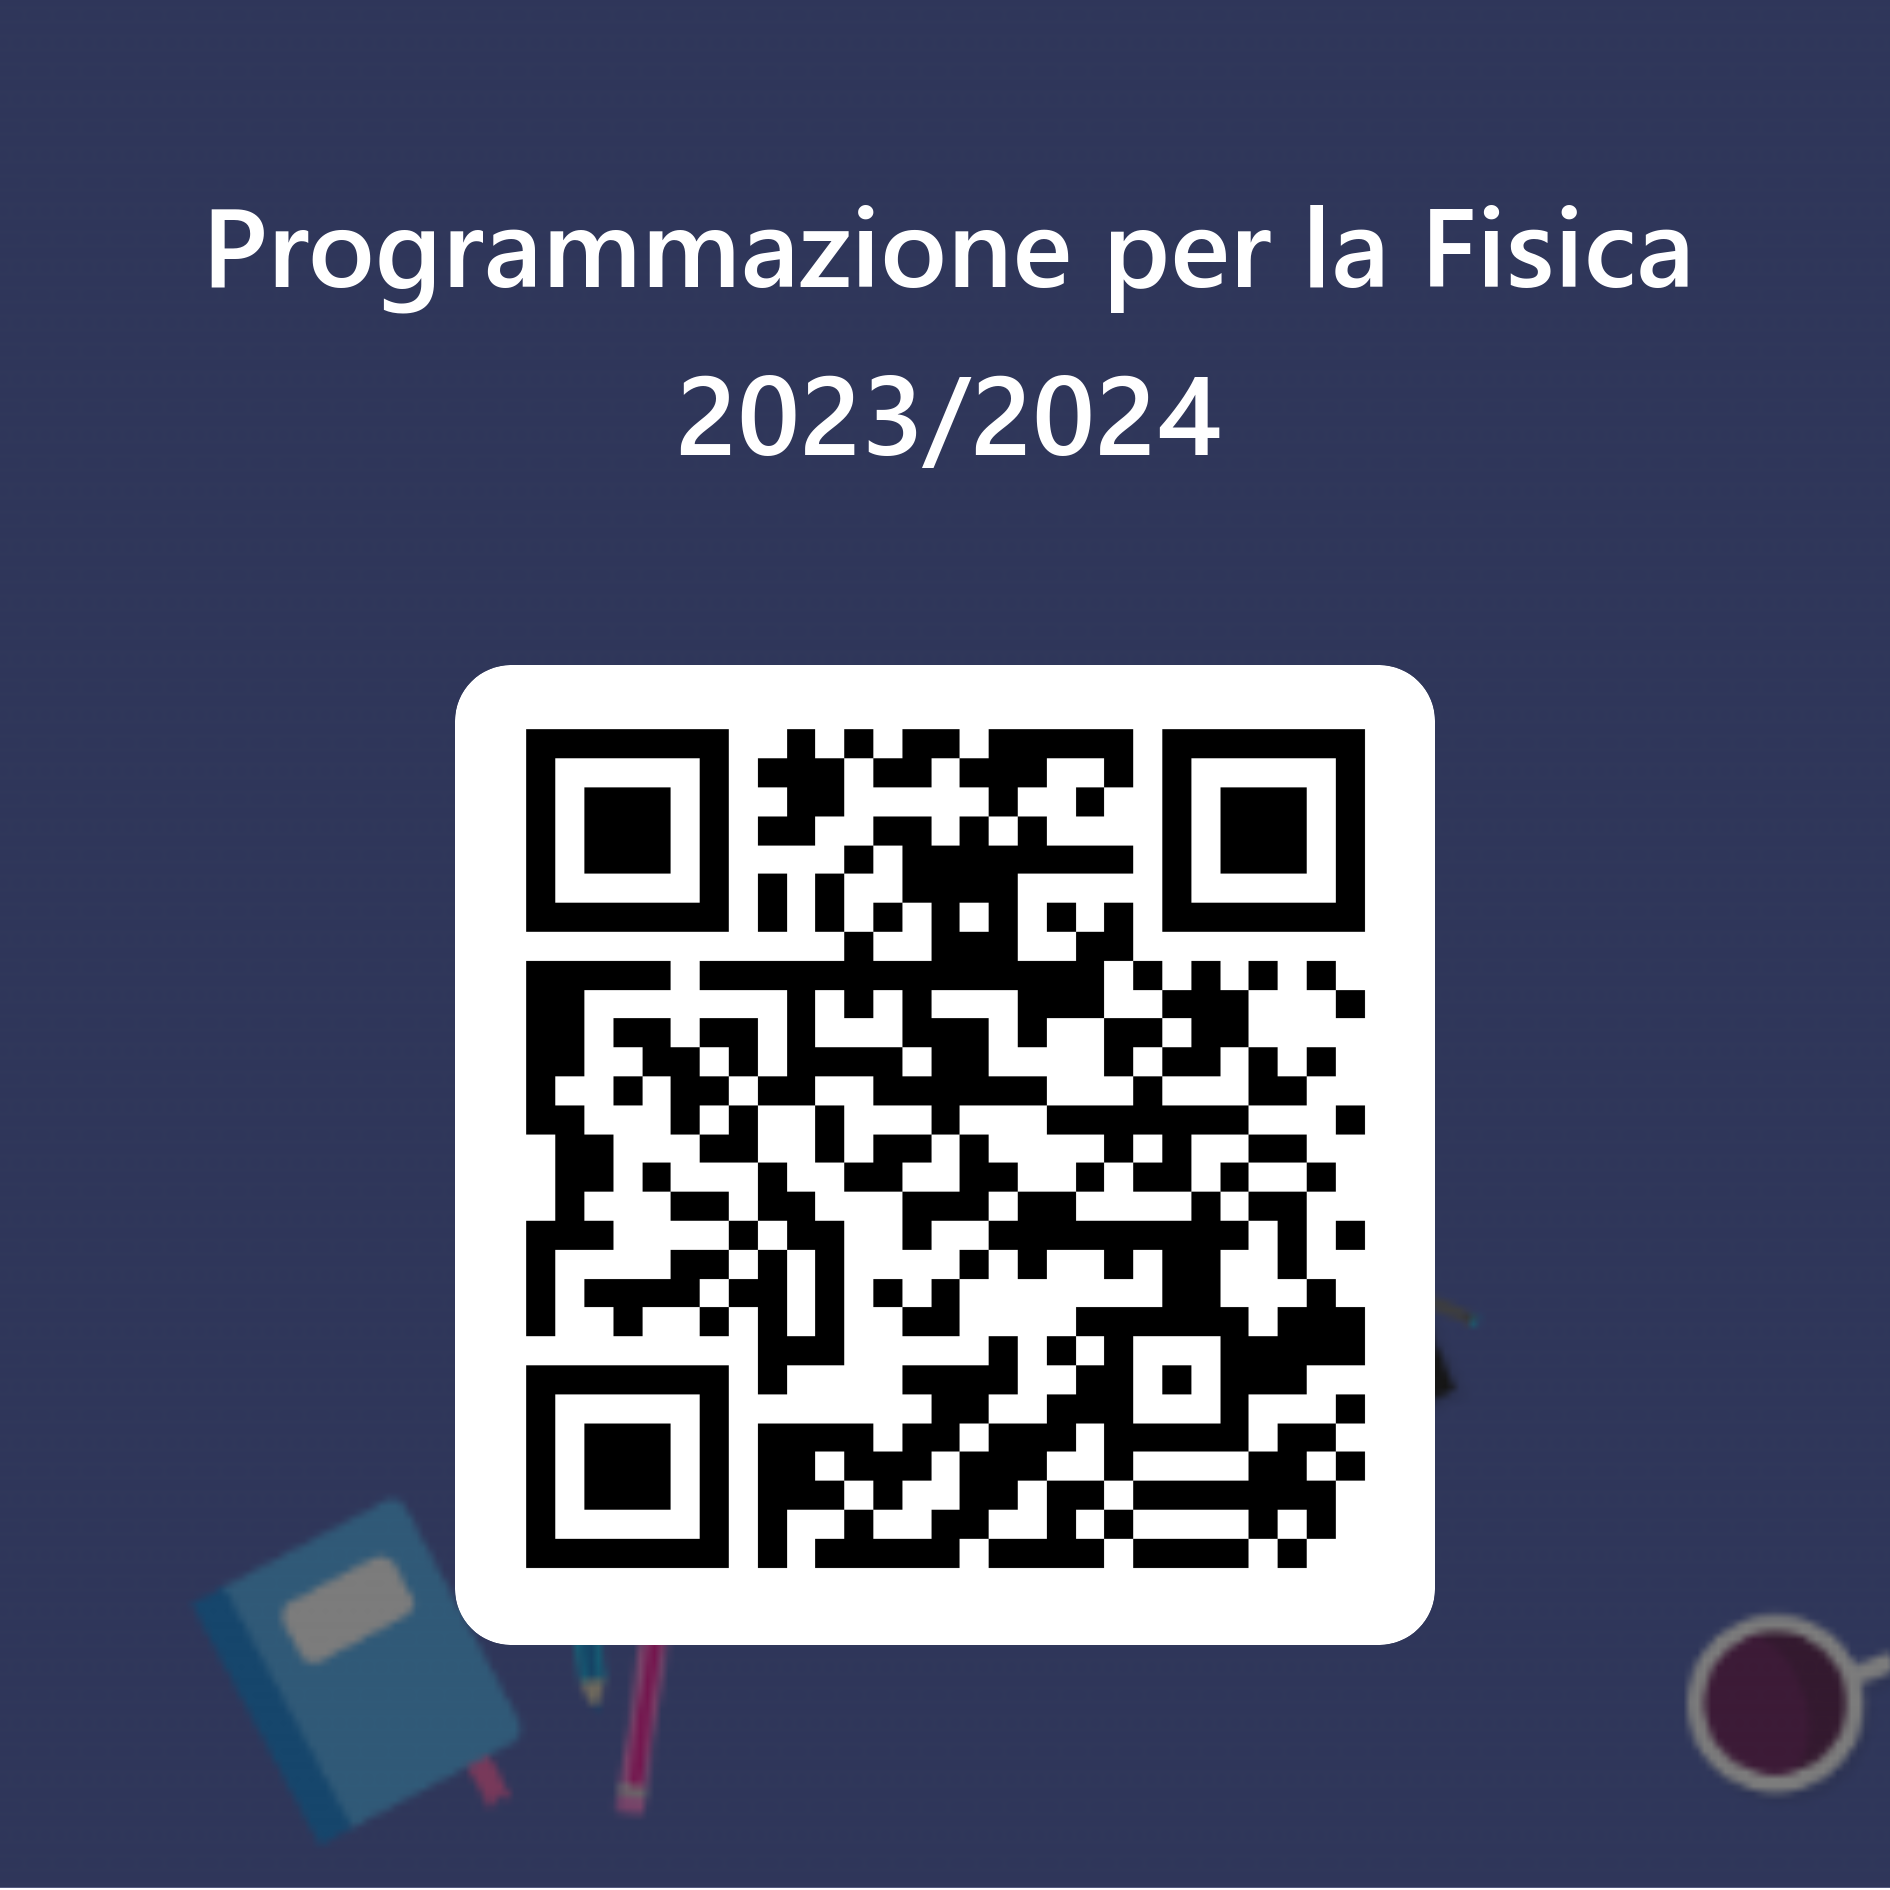
\includegraphics[trim={400 200 400 600},clip,height=.6\textheight]{images/sondaggio-qr.png}
    \vfill
  \end{center}
\end{frame}

\begin{frame}{Materiale di supporto}

  \begin{itemize}[<+->]

  \item Presentazioni, guide, esercizi, \ldots a partire da
    \url{https://github.com/programmazione-per-la-fisica/}
    \begin{itemize}[<.->]
    \item Materiale in parte replicato su Virtuale
    \end{itemize}

  \item Questa presentazione è distribuita in più modalità:
    \begin{itemize}[<.->]
    \item un unico file \code{pdf} aggiornato incrementalmente a ogni lezione,
      disponibile a partire da\\
      {\smaller \url{https://github.com/programmazione-per-la-fisica/pf2023}}\\
      \textbf{non} adatto alla stampa o a prendere appunti (ci sono animazioni)
    \item più file \code{pdf} separati per ogni argomento, caricati su Virtuale
      prima di ogni lezione, adatti alla stampa e a prendere appunti
    \end{itemize}

  \item La presentazione:
    \begin{itemize}[<.->]
    \item ha il testo in inglese, che è la lingua dell'informatica
    \item per me è un ausilio per tenere la lezione
    \item per voi è una sintesi del contenuto del corso, non una dispensa
    \item non può essere la vostra unica fonte per imparare a programmare
    \end{itemize}

  \end{itemize}
  
\end{frame}

\begin{frame}{Bibliografia e risorse consigliate}

  \begin{itemize}

  \item \textit{Learn \Cpp{}}, \url{https://learncpp.com/}: risorsa online con
    tutorial, esempi, esercizi

  \item
    \href{https://isocpp.github.io/CppCoreGuidelines/CppCoreGuidelines}{\textit{\Cpp{}
        Core Guidelines}}: linee guida per il corretto uso del \Cpp{}

  \item B.~Stroustrup, \href{https://stroustrup.com/tour3.html}{\textit{A tour
        of C++}}, 3rd edition (disponibile da ottobre 2022), Addison-Wesley.
    Parte dei contenuti della seconda edizione è disponibile online alla pagina
    \url{https://isocpp.org/tour}

  \item B.~Stroustrup,
    \href{https://stroustrup.com/programming.html}{\textit{Programming:
        Principles and Practice Using C++}}, 2nd edition, Addison-Wesley

  \item B.~Stroustrup, \href{https://stroustrup.com/4th.html}{\textit{The C++
        Programming Language}}, $4^{th}$ edition, Addison-Wesley

  \item B. Stroustrup, \textit{C++ -- Linguaggio, libreria standard, principi
      di programmazione}, IV edizione, Pearson

  \item Come referenza online: \Cpp{} reference, \url{https://cppreference.com/}

  \end{itemize}

  Evitate di consultare risorse, soprattutto online, obsolete o di scarsa
  qualità. Nel dubbio chiedete ai docenti.

\end{frame}

\begin{frame}{Canali di comunicazione}

  \begin{itemize}[<+->]
  \item Virtuale

    \begin{itemize}[<.->]
    \item Usato soprattutto per annunci ufficiali relativi al calendario di
      lezioni e laboratori
    \item Iscrivetevi al più presto
    \end{itemize}
    
  \item Teams

    \begin{itemize}[<.->]
    \item Quest'anno proviamo a mettere a disposizione una chat come strumento
      di comunicazione più agile tra di noi, ad esempio per darvi informazioni
      pratiche durante le lezioni e i laboratori, per chiedere aiuto o
      chiarimenti, ecc.
    \item Per iscrivervi inviate mail a ...
    \end{itemize}

  \item Ricevimento

    \begin{itemize}[<.->]
    \item In presenza o via Teams, su appuntamento
    \item Ma potete anche scrivermi via mail o chat privata Teams
    \end{itemize}
    
  \item Commenti, domande e suggerimenti sono benvenuti in ogni forma e in ogni
    momento
    \begin{itemize}[<.->]
    \item Non aspettate la valutazione finale (che comunque è importante)
    \end{itemize}

  \end{itemize}
  
\end{frame}

\begin{frame}{Modalità d'esame}

  L'esame consiste in due prove:

  \begin{enumerate}

  \item Progetto riguardante l'implementazione di un programma nel linguaggio
    \Cpp{}. Il progetto è svolto in parte durante le ore di laboratorio, in
    parte in autonomia. E' raccomandato lo svolgimento in gruppo (massimo 4
    persone, dipende dalla complessità del progetto).

    Maggiori dettagli verso metà corso, ma potete consultare
    \href{https://github.com/Programmazione-per-la-Fisica/progetto2022}{la
      consegna dell'anno scorso} per avere un'idea.

  \item Colloquio orale riguardante la discussione del progetto e domande
    teoriche e pratiche sugli argomenti svolti a lezione.

    Al colloquio si accede solo con una valutazione sufficiente del progetto.

  \end{enumerate}

  All'orale si porta anche il lavoro svolto durante le esercitazioni di
  laboratorio, a dimostrazione dell'effettivo svolgimento.

\end{frame}

\begin{frame}{Sistemi operativi e strumenti vari}
  \begin{itemize}[<+->]
  \item Il sistema operativo di riferimento è Linux (Ubuntu 22.04)
  \item Forniamo supporto per installare e configurare
      \href{https://github.com/Programmazione-per-la-Fisica/howto/blob/main/other-OSes/WSLGuide.md}{Windows} and
      \href{https://github.com/Programmazione-per-la-Fisica/howto/blob/main/other-OSes/macOSGuide.md}{macOS}
  \item Per scrivere programmi si usa un \textit{\textbf{text} editor}
    \begin{itemize}[<.->]
    \item Noi raccomandiamo \href{https://code.visualstudio.com/}{\textbf{Visual
          Studio Code}}
    \end{itemize}
  \item Imparate a usare strumenti online, in particolare
    \begin{itemize}[<.->]
    \item \href{https://godbolt.org/}{\textbf{Compiler Explorer}}, che useremo
      anche all'orale
    \end{itemize}
  \end{itemize}

\end{frame}

\begin{frame}{Orario primo semestre}
  \begin{itemize}
  \item Lezione/esercitazione: lunedì ore 14-16
  \item Laboratorio: martedì ore 9-13 (M-Z) e 14-18 (A-L), su due
    turni ciascuno, in Aula 2 sede Irnerio
    \begin{itemize}
    \item La partecipazione a Laboratorio è \textbf{obbligatoria}
    \item Indicativamente avremo 3 laboratori il primo semestre e 5 il secondo
    \end{itemize}
  \end{itemize}
\end{frame}

\begin{frame}{Prossimi appuntamenti}
  \begin{itemize}

  \item Lunedì 2/10 ore 14-16 lezione

  \item Martedì 3/10 in base ai turni dei lab, Aula 2 Irnerio
    \begin{itemize}
    \item Installazione/configurazione computer personali
    \item Raccomandato per chi non ha esperienza di programmazione su Linux
    \end{itemize}

  \item Lunedì 9/10 ore 14-16 lezione

  \item Martedì 10/10 in base ai turni dei lab, Aula 2 Irnerio
    \begin{itemize}
    \item Introduzione a Linux/Unix
    \item Raccomandato per chi non ha familiarità con Linux/Unix
    \end{itemize}

  \item Lunedì 16/10 ore 14-16 lezione

  \item Martedì 17/10 in base ai turni dei lab, Aula 2 Irnerio
    \begin{itemize}
    \item Primo laboratorio
    \item Obbligatorio
    \end{itemize}

  \end{itemize}
\end{frame}

\begin{frame}{Course outline}
  \begin{itemize}
  \item<1-> Elements of computer architecture and operating systems
  \item<2-> Introduction to Linux/Unix
  \item<3-> Why \Cpp{}
  \item<4-> Objects, types, variables
  \item<4-> Expressions
  \item<4-> Statements and structured programming
  \item<4-> Functions
  \item<4-> User-defined types and classes
  \item<4-> Generic programming and templates
  \item<4-> The Standard Library, containers, algorithms
  \item<4-> Error management
  \item<4-> Dynamic memory allocation
  \item<4-> Dynamic polymorphism (aka object-oriented programming)
  \item<5-> Elements of software engineering and supporting tools
  \end{itemize}
\end{frame}
